\chapter{Modelos de negocio con software libre}

Ya debe haber quedado claro que el software libre no es necesariamente gratis, aunque, como dijimos previamente, el costo del código tiende a cero, por lo que el modelo de negocios tradicional en la industria del software no puede aplicarse a este tipo de software. Otra característica que surge del modelo de desarrollo de software libre es que es imposible, a diferencia del software propietario, obtener ventajas abusivas por posición dominante (característica conocida comúnmente como ``monopolio''), ya que el código fuente está disponible para cualquier persona o empresa, y ante abusos del grupo de desarrollo se puede producir una división (a veces denominada \emph{fork}) y generar un producto con las mismas características que el original. 

En este capítulo presentaremos algunos de los modelos de negocios que pueden utilizarse en el marco del software libre o de fuentes abiertas, haciendo la aclaración que algunos de ellos pueden superponerse o combinarse en algunos proyectos.

\section{Financiación pública}

Siguiendo un modelo similar al de la financiación de la investigación básica, las instituciones públicas o fundaciones sin fines de lucro pueden proveer apoyo económico a proyectos de software libre. Según las características del proyecto y los objetivos de la institución financiante, puede que la institución participe o no en la gestión del proyecto y desarrollo del software.

Usualmente no busca recuperar la inversión, pero tiene objetivos claros. Por ejemplo, favorecer cierta industria, promover cierta tecnología o estándares, desarrollar herramientas de bajo costo para instituciones públicas, facilitar el acceso a tecnología, etc.

Un caso cercano de este tipo es el desarrollo del sistema operativo Huayra, una distribución GNU/Linux, que es financiado por el gobierno argentino a través de un equipo de desarrollo propio\footnote{Huayra GNU/Linux: \url{https://huayra.educar.gob.ar/}}. Esta distribución, y algunas aplicaciones desarrolladas por el mismo equipo, es incluida en las computadoras del Plan Conectar Igualdad, que distribuye computadoras portátiles a estudiantes de escuelas secundarias públicas de todo el país\footnote{Plan Conectar Igualdad: \url{https://conectarigualdad.edu.ar/}}.

\section{Financiación privada}\label{sec:finPrivada}

Algunos proyectos de software libre son llevados a cabo o financiados por empresas, es decir, instituciones con fines de lucro. En forma similar a la financiación anterior, tanto los objetivos como el involucramiento de la empresa en la gestión y desarrollo del proyecto pueden variar.

Un ejemplo interesante de estos dos tipos de financiación, y de cómo esta va variando a lo largo de la vida de un software, es el de la suite de oficina OpenOffice: el software privativo llamado StarOffice, fue adquirido en 1999 por la empresa Sun Microsystems para uso interno, pero en 2002 lo liberó como software libre con el nombre de OpenOffice para competir con la suite Microsoft Office y promover la utilización del estándar libre de documentación ODF (siglas de \emph{Open Document Format}. En 2010 la empresa fue adquirida por Oracle Corporation y al año siguiente se informó que no se continuaría financiando el proyecto OpenOffice, el cual se donó a la Fundación Apache, que lo sigue desarrollando bajo el nombre de Apache OpenOffice\footnote{Apache OpenOffice: \url{https://www.openoffice.org/es/}}. Mientras tanto, un grupo independiente de la comunidad realizó un \emph{fork} y creó la fundación The Document Foundation, la cual, en base al código de OpenOffice, desarrolla actualmente la suite LibreOffice\cite{watkins18}\footnote{LibreOffice: \url{https://es.libreoffice.org/}}.

En las últimas décadas han surgido cooperativas (empresas gestionadas por sus trabajadores\footnote{Formalmente una cooperativa es una asociación autónoma de personas que se han unido
voluntariamente para hacer frente a sus necesidades y aspiraciones económicas, sociales o culturales comunes por medio de una empresa de propiedad conjunta y democráticamente controlada.}) dedicadas a la tecnología basada en software libre o que desarrollan software libre. Lo mencionamos como un caso especial debido a que la filosofía del movimiento de software libre y los principios cooperativos tienen muchos puntos en común, tales como la pertenencia abierta y voluntaria a la comunidad o empresa, el control horizontal por parte de sus miembros, el compromiso con la comunidad, el compartir el conocimiento y el aporte del saber de cada miembro de la comunidad\cite{monk14}.

\section{Financiación por quien necesita mejoras}

Cuando un/a usuario/a o empresa requiere mejoras o funcionalidades específicas en un software libre puede financiar a un grupo (de la comunidad o ajeno a ella) para que las desarrolle. Cabe destacar que si el software mejorado resultante es para uso interno de la empresa no es requisito la redistribución libre del código generado, aunque el original tenga una licencia robusta. Sin embargo, si el software se redistribuye solo o como parte de un producto o servicio, una licencia robusta exigirá que la mejora (aún siendo pagada por la empresa) sea distribuida con la misma licencia que el código original. También es costumbre compartir el nuevo código aunque no sea un requisito legal, como aporte a la sociedad y en agradecimiento por el software original.

Este tipo de financiación permite que software desarrollado globalmente beneficie al mercado local, ya que usualmente se contrata a equipos de trabajo locales por una cuestión de cercanía, afinidad cultural y mayor simplicidad en los procesos comerciales y legales.

Una variación de este tipo de financiación es el aporte de tiempo de trabajo de desarrolladores/as de una empresa a un proyecto de software libre. Un grupo de desarrolladores/as de una empresa dedica su tiempo de trabajo, total o parcial, a desarrollar componentes o realizar mejoras a un software libre, formando parte de la comunidad. Este tiempo es pagado por la empresa como parte del sueldo de los/as desarrolladores/as. Este fue el caso de Corel, que en 1999 dedicó un equipo de ingenieros/as al proyecto Wine\footnote{Wine (\emph{Wine Is Not an Emulator}) es un software libre que implementa las API de Microsoft Windows en Linux, permitiendo que  aplicaciones desarrolladas para Windows se ejecuten en un sistema Linux sin necesidad de ser recompiladas. \url{https://www.winehq.org/}} para que le agregaran funcionalidades que permitiría que las aplicaciones de Corel, tales como WordPerfect, CorelDRAW y Quattro Pro, correr en Linux en forma eficiente y sin necesidad de reescribir el código de las aplicaciones~\cite{corel99}.

\section{Financiación por consultoría}

Este tipo de negocios es similar al anterior, pero generalizado a cualquier tipo de actividad que requiera el cliente. Tanto puede ser realizar mejoras al software (arreglo de errores específicos, agregado de funcionalidades) como análisis para determinar si el software es el adecuado para la empresa o actividades de instalación de software particularmente complicado o en ambientes complejos.

El fundamento de este modelo de negocios es que las empresas usuarias de software libre generalmente ante un problema del software no pueden depender de los tiempos de la comunidad sino que requieren una solución inmediata. El firmar acuerdos de servicio técnico con empresas proveedoras le permite garantizar ciertos tiempos de respuesta adecuados para asegurar la continuidad del negocio.

Este es el enfoque de negocios de muchas de las empresas basadas en software libre más exitosas. El mayor ejemplo de esto es Red Hat\footnote{Red Hat: \url{https://www.redhat.com/es}}, cuyo servicio de consultoría basado en una distribución del sistema operativo GNU/Linux, comenzando en 1993 la llevó a ser una empresa valuada en 33 mil millones de dólares, precio al cual la adquirió IBM en 2018.
 
\section{Financiación por servicios web}

Recientemente, y dependiendo de sus características, muchos proyectos de software libre ofrecen tanto una versión para instalar en los equipos de los/as usuarios/as como una versión en la nube, que provee servicios web con ciertos esquemas de pago (puede haber un servicio básico gratuito y mayores precios según los servicios provistos). Lo que se cobra en este caso no es el software, sino los servicios web (almacenamiento, gestión de usuarios, etc.).

Cabe notar que una ventaja de este enfoque comercial es que el/la usuario/a no necesita estar pendiente de las nuevas versiones, el software en la web se actualiza a medida que aquellas van siendo liberadas. Por otro lado, al ser software libre, si el/la usuario/a no está conforme con los servicios provistos puede descargarlo e instalarlo en sus equipos o en los equipos de un proveedor de servicios de nube y continuar usándolo sin mayores costos.

Un ejemplo de este tipo de negocio es Moodle\footnote{Moodle: \url{https://moodle.org/}}, la plataforma de gestión de clases que utilizamos en esta asignatura. La instancia que utilizamos está instalada en los servidores del centro de cómputos de la UTN-FRC, pero instituciones que no tengan estas facilidades pueden adquirir diferentes planes y utilizar Moodle en la nube. En la Fig.~\ref{figMoodle} se muestran los diferentes planes al día de hoy. 

\begin{figure}[h!]
\centering
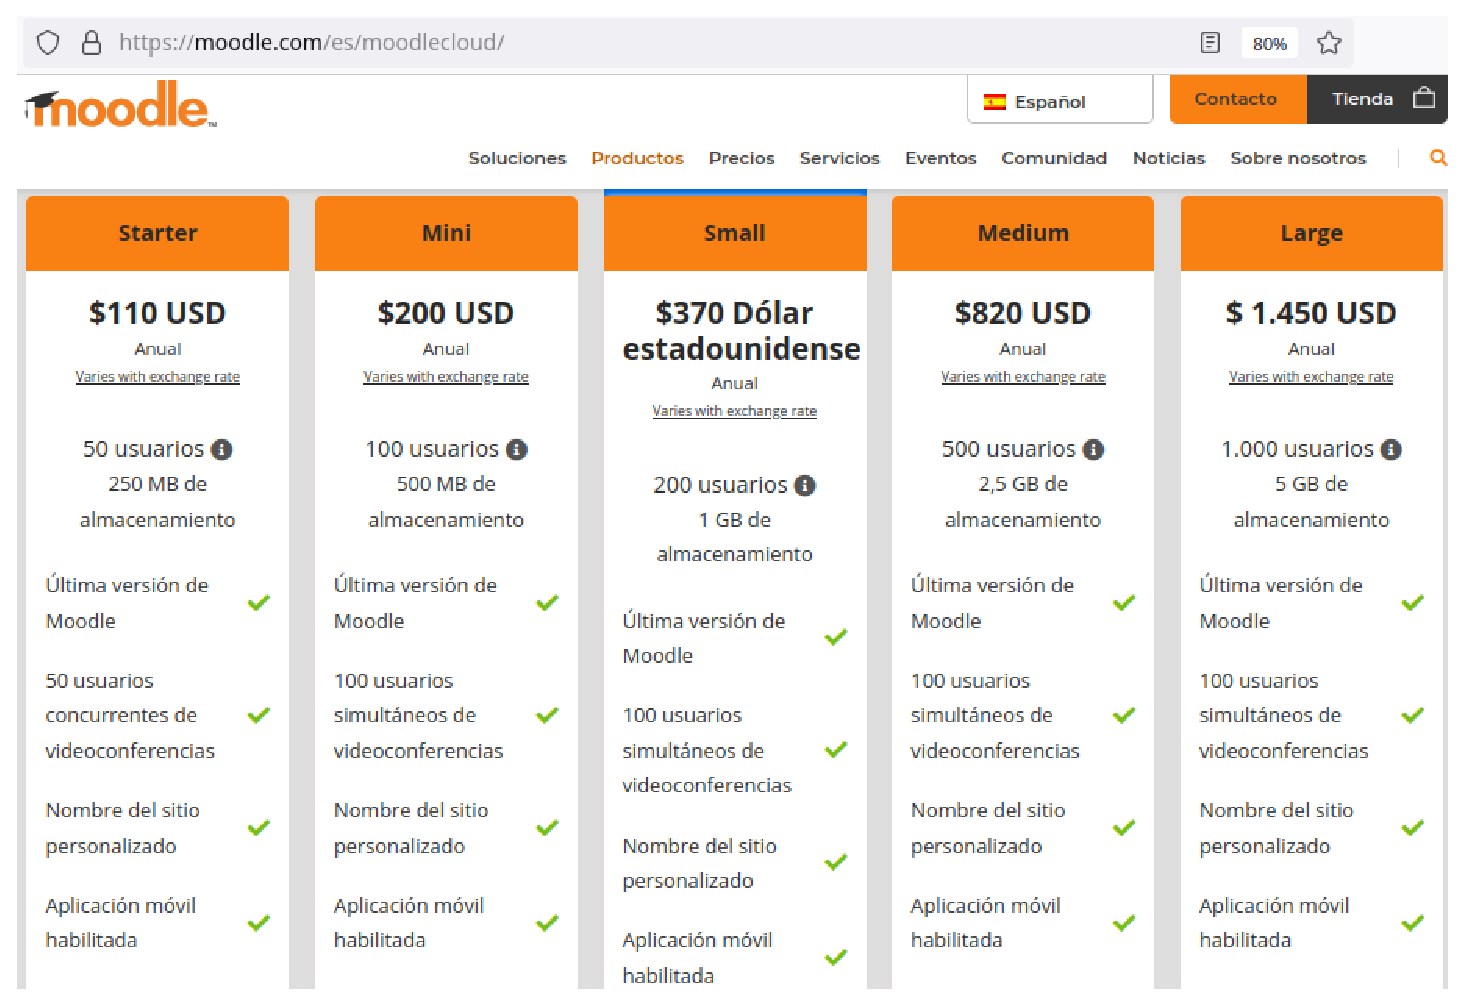
\includegraphics[scale=.5]{imagenes/moodle.eps}
\caption{Planes de servicio de Moodle en la nube. Precios en dólares al 23/02/2022.}
\label{figMoodle}
\end{figure}


\section{Financiación por productos relacionados}

Ya que no es razonable vender el código, una fuente de financiación de proyectos libres es la venta de productos asociados, ya sean tangibles o intangibles.

\begin{itemize}
\item {\bf \emph{Merchandising}:} Es común la venta de remeras, gorras, calcos y otro material sobre proyectos o comunidades de software libre. Para que los fondos obtenidos de esta manera beneficien a la comunidad que desarrolla el software es usual que la marca, nombre y/o logo del proyecto estén protegidos legalmente. Por ejemplo, Linux es una marca registrada de Linus Torvalds y Firefox es marca registrada de la Mozilla Foundation, así como el logo del navegador.

\item {\bf Formación:} Cursos, entrenamiento, manuales y libros sobre software libre también son fuentes de ingresos para las comunidades de software libre. Aunque cualquier persona o empresa puede desarrollar actividades de formación sobre un proyecto de software libre, usualmente quienes están involucrados en la comunidad están en ventaja para hacerlo, ya que poseen un conocimiento profundo del software en cuestión.
 
\end{itemize}

Como ejemplo de esto último mencionamos en particular a la editorial O’Reilly, que publica libros sobre diferentes proyectos de software libre, beneficiando generalmente a sus creadores originales. Debe notarse, además, que muchos de sus libros a su vez tienen licencias libres\footnote{O'Reilly Open Books: \url{https://www.oreilly.com/openbook/}}.

\section{Licenciamiento múltiple}

En algunos casos, para financiar el proyecto libre el producto de software se distribuye bajo dos licencias o más, siendo al menos una de ellas libre y las otras propietarias. Generalmente las versiones bajo licencia propietaria tienen funcionalidades que la versión libre no tiene (pasado un tiempo esas funcionalidades se agregan a la versión libre, pero quienes pagan por la licencia propietaria pueden acceder antes a estas funcionalidades).

Usualmente las versiones bajo licencia propietaria incluyen servicios de consultoría y tiempos de respuesta rápidos a solicitudes del/la usuario/a.

Un clásico ejemplo, entre muchos, es la base de datos MySQL\footnote{MySQL: \url{https://www.mysql.com/}} que utiliza la licencia GPL para su \emph{Community Edition} y una licencia propietaria de Oracle para su versión comercial.

\section{Financiamiento por donaciones}

Algunos proyectos de software libre se financian (al menos parcialmente) a través de donaciones de particulares y empresas. Para facilitar este tipo de financiación se han creado fundaciones que gestionan las finanzas del proyecto (como vimos en la sección~\ref{sec:finPrivada}), aunque esto no es requisito y dependerá de los montos de donaciones que se manejan en cada proyecto.

\section{A modo de cierre}

Hemos visto en este capítulo diferentes modos de financiar (total o parcialmente) un proyecto de software libre. Cabe aclarar que estos modelos de negocios no son excluyentes, muchas comunidades se financian a través de una combinación de estos.



%\section{Impacto sobre las Situaciones de Monopolio}
%
%
%Cualquier iniciativa dedicada a romper una situación donde un producto domina claramente el mercado estará destinada a producir más de lo mismo: si tiene éxito, vendrá otro a ocupar ese hueco y en breve habrá otro dominante. Solo los cambios tecnológicos producen durante un tiempo la inestabilidad suficiente como para que nadie domine claramente.
%El problema no es que haya un producto dominante, sino que haya solamente una empresa que lo ofrezca al mercado. El SW libre ofrece la alternativa a esa situación.
%Lo saludable es que cualquiera sea el producto, muchas empresas puedan competir para proporcionarlo, mejorarlo, adaptarlo y ofrecer servicios alrededor de él.
%
%\subsection{Elementos que favorecen a los productos dominantes}
%
%{\bf Formato de datos:  } cuando mucha gente utiliza un formato de dato dado, la presión para usarlo es enorme.
%
%{\bf Cadenas de distribución: } cuando el producto es dominante es fácil su distribución porque todas las cadenas lo buscan para poder ofrecerlo. Si el producto es minoritario le resulta difícil acceder a su comercialización y llegar a los usuarios.
%
%{\bf Marketing: } el boca a boca es una gran propaganda, cuando son muchos los que lo usan. 
%
%{\bf Inversión en formación: } una vez aprendido el uso de una herramienta, se está muy motivado para no cambiar. Además, usualmente esa herramienta es la que domina, por lo que es más fácil encontrar material y personas que ayuden a aprenderla.
%
%{\bf Software preinstalado: } el usuario lo quiere. Además, el SW que viene preinstalado es el más utilizado.
%
%\subsection{El mundo del software propietario}
%
%En este mundo, la aparición de un producto dominante en un segmento cualquiera equivale a un monopolio por parte de la empresa que lo produce.
%La empresa tiene gran control sobre el producto, ellos marcan su evolución, su calidad, etc. 
%Esta situación hace aparecer los peores efectos económicos del monopolio, entre ellos la falta de motivación de la empresa líder para acercar el producto a las necesidades de sus clientes, ya que están cautivos.
%
%\subsection{La situación del software libre}
%
%Con el SW libre, un producto dominante no se traduce en monopolio de la empresa. Cualquier empresa puede trabajar en él, mejorarlo, adaptarlo a las necesidades del cliente y ayudar a su evolución. Muchos querrán trabajar en esta mejora y si la empresa que lo desarrolló en primera instancia quiere permanecer en el negocio tendrá que competir contra todas ellas y estará muy motivada para hacer evolucionar al producto. Naturalmente tendrá la ventaja de un mejor conocimiento del programa. 
%Los usuarios retoman el control.
%Como ejemplo de productos libres que son dominantes en su sector se puede nombrar Apache y las distribuciones de GUN/Linux.
%
%\subsection{Estrategias para constituirse en monopolio con software libre}
%
%Son estrategias comunes a otros sectores económicos, pero una es específica del mercado del SW: {\bf la aceptación de productos certificados por terceros.}
%Cuando una empresa quiere distribuir SW que funcione en combinación con otras aplicaciones, es común “certificar” la combinación. El fabricante se compromete a ofrecer servicios (actualización, soporte, resolución de problemas) sólo si el cliente está usando el producto en un entorno certificado por él. Si en este segmento la certificación es importante, estamos ante una nueva situación de monopolio.
%Las situaciones monopólicas no son fáciles de conseguir, y para conseguirlas se debe utilizar mecanismos “no informáticos”.
%
%
